Метод главных компонент во всех библиотечных реализациях называется РСА, существует для понижения размерности.

\textbf{Мотивация}\\

Вспомним зачем вообще интересно понижать размерность.
\begin{enumerate}
    \item В задачах ML размерность данных может быть очень большой. Например, миллионы признаков, особенно когда это разреженные признаки - становится сложно работать.
    \item Такие данные сложно визуализировать, сложно обучать модели.
    \item Чтобы снизить размерность, нам требуется использовать какой-то механизм, который по-хорошему все-таки воспроизводим.
\end{enumerate}


РСА - линейный способ понижения размерности, который интуитивен и используется широко на практике. Зачем нам может понадобиться матричное разложение на практике?
Матрица объект-признак $X$ может быть приближена произведением двух матриц меньшего ранга:

$$X_{l,d} \approx U_{l, k}V_{k,d}^T$$

Где размерность $k < d, l$. В таком случае мы можем сказать, что у нас есть матрица перехода и матрица, которая кодирует всю информацию. И теперь использовать приближение меньшего ранга для всех наших данных, потеряв часть информации, но используя меньше признаков. \\

Такое разложение можно построить с помощью минимизации $\|X - UV^T\| \to \min$. (Тут норма или норма Фробениуса, или какая-нибудь еще).\
РСА нам говорит, что мы можем матрицу признаков разложить на произведение трех матриц: $X = U\Sigma V^T$.

В этом выражении матрицы $U, V^T$ являются ортогональными матрицами, а $\Sigma$ - диагональная матрица. Можем сказать, что $k$ ненулевых признаков остаются ненулевыми и значимыми. Получаем это с помощью взятия $k$ диагональных элементов матрицы $X$ и соответствующих им столбцов в матрицах $U, V$. Таким образом при перемножении получается итоговая матрица меньшей размерности, итоговый ранг равен $k$.

\begin{center}
    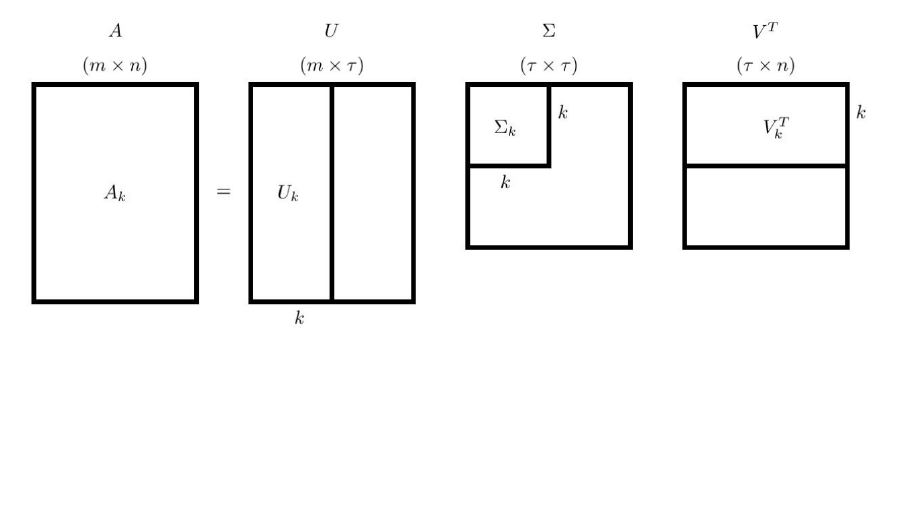
\includegraphics[scale=0.7]{images/12_1.png}
\end{center}

\begin{theorem}[Эскарта-Янга]
$SVD$ дает наилучшую аппроксимацию нашей изначальной матрицы

$$X_k = U_k\Sigma_k V_k^T$$
$$\forall B_k : \rk(B_k) = k$$
$$\|X - B_k\|_F \geqslant \|X - X_k\|_F$$
Где $B_k$ -- матрица ранга $k$, полученная не по SVD разложению.
\end{theorem}

\textit{Плюсы:}

\begin{enumerate}
    \item Так как используемые отображения линейны, значит и РСА - линейная модель, а значит будет работать достаточно быстро
    \item преобразование, из которого можно будет вернуться в исходное пространство, пусть и с какими-то потерями (перешли в другое пространство с помощью $U_k\Sigma_k$, вернулись с помощью $V_k^T$).
\end{enumerate}

Так как у нас матрицы $U, V$ ортогональны, давайте перетасуем все величины на диагонали матрицы $\Sigma$ таким образом, чтобы они шли по убыванию. Первые $k$ элементов -- самые большие величины, которые позволяют описать данные наилучшим способом в $k$-мерном пространстве с точки зрения нормы Фробениуса. \\

\textbf{Интуитивная интерпретация PCA}\\

Представим себе облако точек. 

\begin{center}
    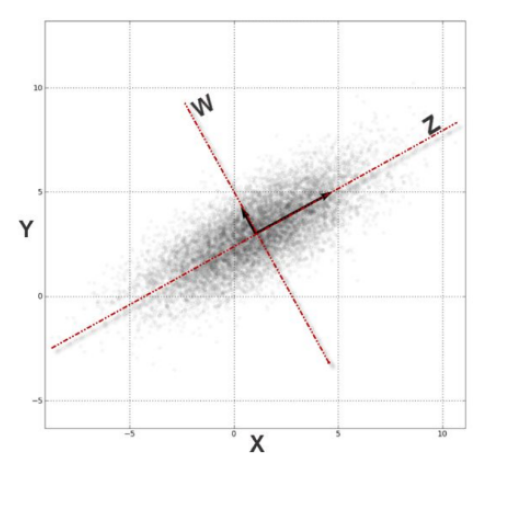
\includegraphics[scale=0.7]{images/12_2.png}
\end{center}

По сути мы переходим в базис главных компонент, которые можно заметить интуитивно: первая главная компонента - вдоль которой дисперсия максимальна (большая ось эллипса, определяем с точностью до направления), вторая и последующие главные компоненты будут ортогональны первой главной компоненте (так как мы помним, что компоненты матрицы ортогональны). \\

Мы работали на картинке в двумерном пространстве, получили две главные компоненты, теперь если мы захотим снизить размерность пространства, нам надо будет выбрать первую главную компоненту, чтобы не потерять максимальное количество информации.\\

\begin{note}
\textit{Вопрос, который любят задавать на собеседованиях:}
Каждая новая компонента смотрит в направлении максимальной дисперсии в оставшемся подпространстве, в котором мы теперь работаем. Все векторы ортогональны друг другу.
Когда РСА выдаёт нам с ошибкой главные компоненты?\\


Понятно, что с точностью до направления они и так неоднозначно могут быть определены, но если у нас есть симметричность в данных - например, они лежат на поверхности сферы, тогда главные компоненты могут быть любые. То есть мы берем любые $k$ ортогональных векторов, где $k$ -- размерность пространства.
\end{note}

\begin{example}[Проблема]
Как правило данные к нам приходят вообще из разных источников. Например, в выборке могут быть признаки: рост, вес, зарплата в долларах, зарплата в рублях и ещё $50$ разных признаков. И мы можем обнаружить, что различные величины находятся в различных шкалах. Допустим рост в см от $50$ до $200$, вес от $40$ до $140$, а зарплата от $10$ до $10000$ в долларах и тд. Тогда получается, что чем больше разброс у того или иного признака, тем больше вдоль этого направления будет дисперсия, тем больше он на себя будет оттягивать внимания у каждой следующей главной компоненты. Это неправильно, так как вместо того, чтобы смотреть на линейные подрпространства и искать информативные комбинации исходных признаков, мы будем смотреть на признаки с большей дисперсией в используемых шкалах.
\end{example}

\begin{note}[Важно]
В принципе проблема та же, с которой мы боролись $L_2$-регуляризацией. Чем больше разброс какого-то признака, тем меньше нам нужны веса для того чтобы моделировать поведение нашей модели. Поэтому если не нормировать данные перед РСА, РСА не даст адекватный результат.
\end{note}

Повторим, что шаг $X_k = U_k \Sigma_k$ даёт понижение размерности, а шаг $\overline{X} = X_kV_k^T$ возвращает нас в исходное пространство.

В принципе, нам может быть интересно посмотреть на отклонение $\overline{X}$ от $X$.

\begin{example}
    Рассмотрим:
    \begin{center}
    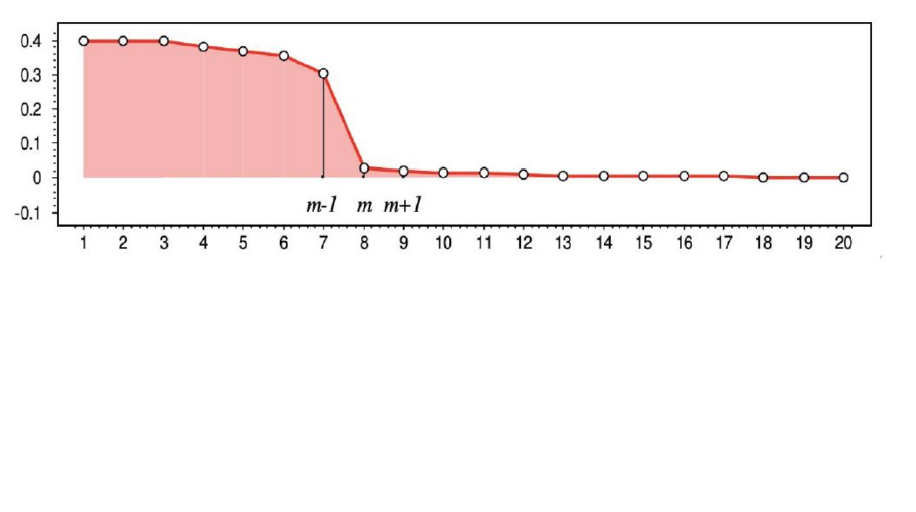
\includegraphics[scale=0.7]{images/12_3.png}
    \end{center}

    В какой-то момент количество дисперсий значительно падает, это значит, что мы нашли линейное подпространство, которое описывает $99\%$ наших данных. И, на самом деле, это как раз то количество главных компонент, которые нужно использовать.
\end{example}

Собственно, на практике мы сначала строим $PCA$ такой же размерности, как и наше пространство (или как максимальное число компонент, которые вообще чисто физически возможно взять). Дальше смотрим на график как из примера выше и уже берем только нужное нам количество.

